\documentclass[11pt,twocolumn]{article}

\usepackage[utf8]{inputenc}
\usepackage{amsmath}
\usepackage{amssymb}
\usepackage{parskip}
\usepackage{mathtools}
\usepackage{verbatim}
\usepackage{color}
\usepackage{graphicx}
\usepackage{caption}
\usepackage{listings}
\usepackage{xcolor}
\usepackage{subcaption}
\usepackage[noend,linesnumbered]{algorithm2e}
\usepackage{setspace} 
\usepackage{enumerate} 
\usepackage{amsthm}
\newcommand{\lra}{\Leftrightarrow}
\newcommand{\join}{\bowtie}
\newcommand{\select}{\sigma}
\newcommand{\project}{\pi}
\newcommand{\distinct}{\delta}
\newcommand{\Schema}{\Sigma}
\newcommand{\ra}{\rightarrow}
\newcommand{\la}{\leftarrow}
\newcommand{\q}{\quad}
\newcommand{\tbf}{\textbf}
\lstset { %
    language=C++,
    backgroundcolor=\color{black!5}, % set backgroundcolor
    basicstyle=\footnotesize,% basic font setting
}


\usepackage[left=1in,right=1in,top=1in,bottom=1in]{geometry}

\DeclarePairedDelimiter{\ceil}{\lceil}{\rceil}

\usepackage{amssymb}

\let\oldemptyset\emptyset
\let\emptyset\varnothing

\newcommand\NV[1]{**NV #1 ** }
\newcommand{\code}{\lstinline}



\begin{document}

\title{Project Report}
\author{Konstantinos Zarifis \quad Jules Testard \quad Michael Barrow}
\maketitle

\section{Introduction}

We present here an implementation of a data flow analysis module for the C++ LLVM compiler. Our implementation includes four types of analyses 1) Pointer Analysis 2) Constant Propagation 3) Available Expressions 4) Range analysis. All analyses are made on a function scope. We first present our interface followed by detailed description of the implementation of each analysis.


\section{The interface}

We have designed the interface with the client analysis developper in mind.
It is built to be clear, understandable, easy to use and easy to extend. The focus has been put on clarity and extensibility rather than performance. Indeed, to build a basic client analysis, only two classes have to be extended and five short virtual methods overridden. We go over each component of the interface implementation. For each component, we describe how a client can use the interface and quickly build his own analysis.

\subsection{The Context Flow Graph}
The first aspect of the dataflow analysis we implemented was its internal representation, the context flow graph.
We wanted to model our dataflow analysis following closely the pseudo code found in the lecture notes. We noticed that the LLVM library provided its own graph implementation in the form of \code{BasicBlocks} and \code{Instructions}. However, we found the stucture of the LLVM library graph too complex and it did not offer the possibility to store the analysis information (which we call \emph{flow}) within. Therefore, we created our own graph structure which is defined in listing \ref{CFG}.

\begin{lstlisting}[caption=Context Flow Graph, label=CFG]
typedef struct ListNode {
  int index;
  vector<ListEdge*> incoming;
  vector<ListEdge*> outgoing;
  Instruction *inst;
  ListNode(int idx){
    index = idx;
  }
} ListNode;

typedef struct ListEdge{
  Flow* flow;
  ListNode* source;
  ListNode* destination;
  ListEdge(ListNode* src, ListNode* dst){
    source = src;
    destination = dst;
    flow = new Flow();
  }
} 
\end{lstlisting}

Each node can have multiple incoming and outgoing edges and represents an instruction in the program. An index has been added to more easily identify the instruction within the program. However, the flow is store only in the edges, in accordance with the algorithm seen in the lecture notes. A convenient method allows the user to display the graph in \code{JSON} format. Finally, the clients do not need to be aware of the graph structure, as it is only used by the class they are going to extend.

\subsection{The Flow Class}

The \code{Flow} class is the way we represent the information computed by analyses which use our interface. Any client must create his own class which will extend the \code{Flow} class. The class does not contain any container for the computed, leaving this job entirely to the subclass. This decision allows the class to be very flexible and allow just about any kind of data model for the computed information, although this information is most often represented a map from variables to analysis-specific domain elements. The subclass is however required to override a number of virtual C++ functions.

The \code{Flow} class includes a lot of the functionality from the lattice operators seen in class. The first method overriden by the client is the \code{Flow* join(Flow* other);} method, which joins the \code{this} flow and the \code{other} flow together. The \code{this} flow and the \code{other} flow objects are not altered by this method, rather a copy of their merged information is outputted. The client must also override the \code{bool equals(Flow* other)} and \code{void copy(Flow* other)} which allow comparison and duplication, respectively. The \code{void copy(Flow* other)} method should be read as "copy flow \code{other} into \code{this}", and therefore does not have a return type.

In all of the overridden versions of these methods, the client will have to cast the input \code{Flow*} type to an instance of his client class in order to have access to all the fields required to implement these methods accurately. The type casting can happen safely, because it will always be the case when those methods are called, that the incoming flow's actual type will be that of the client subclass. For increased readibility, we initially wanted the $copy$ and $equals$ methods to be implemented through operator overloading. However, we realized that this is not possible, given operator overloading restricts the input to be a constant pointer and disables casting.

The last method the client must override is the \code{string jsonString()} method which allows the output of the flow in \code{JSON format}. The class defines two constants strings, called \code{"top"} and \code{"bottom"} and a member called \code{basic}, which is only allowed to be empty or have these two values. The \code{jsonString()} method will output \code{"top"} or \code{"bottom"} if and only if the basic string is non-empty, regardless of the analysis, which help clarify the flow representation when outputed in \code{JSON} format.

\subsection{The Static Analysis Class}

While the \code{Flow} class represents the information computed by the dataflow analysis, the \code{Static Analysis} implements the analysis itself. It must also be extended by clients. The \code{Static Analysis} class implements most of the effort required for an analysis, leaving the client class focusing on the flow function implementation.

The \code{StaticAnalysis} class has the responsibility of building the Context Flow Graph, which it does in the \code{void builCFG(llvm::Function &F)} method. Recall that our analysis are made on a function scope. This method will build the graph corresponding to the LLVM function given as argument. When analysis multiple procedures, multiple instances of the Analysis class are created. More details about this are discussed in the next section.

The most important feature of the \code{StaticAnalysis} class is the \code{void runWorklist()} method, whose C++ implementation can be seen on listing \ref{worklist}. This class has been made on purpose extremely similar to the worklist algorithm seen in class. Next, we go over the important methods used by this class.

The \code{void initializeEdgeFlowToBottom()} function has a dual functionality. First, it makes sure the edge flow is initialized to bottom at the start of the analysis. Second, it ensures that the C++ type of the flow used by algorithm is that of the client analysis subclass. When the client extends this class, in his constructor he must initialize the two \code{Flow*} objects \code{top} and \code{bottom} to instance of the client analysis's \code{Flow*} subclass. Next, the \code{Flow* initialize()} method must to be overridden. This method returns a copy of the \code{bottom} flow. When the  \code{void initializeEdgeFlowToBottom()}, it will call \code{Flow* initialize()} on all edge flows in the graph. The method \code{void addAllNodesToWorklist()} is pretty self explanatory.

The \code{Flow* mergeFlowFromIncoming()} method gets all of the flows from the incoming edges of the current node and joins them together using the \code{Flow* join()} method. Note that given all \code{Flow*} objects are instance of the client subclass, through polymorphism the \code{Flow* join()} method that will be called will be that of the client subclass.

Next, the \code{Flow* executeFlowFunction()} method outputs the \code{Flow*} corresponding to the input \code{Flow*} and \code{Instruction*}. This method must be overridden by the client. Inside this function, this client is expected to implement the functionality for every flow function. This leaves the client very free in the way he intends to implement flow functions.

The last part of the worklist algorithm updates the flows of the output edges. Notice that given two consecutive nodes, the outgoing edge for the first node and incoming edge of the second node are the same object (by updating one, you update the other). This section relies on the client interfaces implementing the \code{Flow* join()}, \code{bool equals()}, \code{void copy()} methods correctly.

\begin{lstlisting}[caption=Worklist Algorithm, label=worklist]
void StaticAnalysis::runWorklist() {
  queue<ListNode*> worklist;
  
  initializeEdgeFlowToBottom();
  addAllNodesToWorklist(worklist);
  
  while(!worklist.empty()){
     ListNode* current = worklist.front();
     
     Flow* in = 
     mergeFlowFromIncoming(current);
     
     Flow* out = executeFlowFunction(
     	in,current->inst);
     
     for(unsigned int i = 0 ; i < 
     	current->outgoing.size(); i++) {
       
       Flow* new_out = out->join(
       current->outgoing[i]->flow);
     
       if (!(new_out->equals(current
       ->outgoing[i]->flow))){
     
         current->outgoing[i]->f
         low->copy(new_out);
     
         worklist.push(current->
         outgoing[i]->destination);
       }
     }
    worklist.pop();
  }
}
\end{lstlisting}

\subsection{The AnalysisPass}

Until now, it has been assumed that the LLVM code we want to analyze was given. We actually require the client to write an \code{LLVM::Pass} to perform the analysis. The user is then required to use the LLVM \code{opt} program with the \code{-analyze} flag on the pass he creates to output the computed information. Given our analyses all use function scope, the \code{Pass} should create one analysis object per function in the LLVM module. Notice that the client is not required to extend any class, but an example \code{Pass} is provided as a guideline. Finally, noticed that in our design, it is possible for a single pass to handle multiple analyses, if required. We believe extending our analysis to module scope would be easy, given the flexibility of our framework. In order to extend our scope, we only need to extend our Context Flow Graph to add edges from caller to callee functions (in addition to branching and jumps).

\section{Pointer Analysis}

\begin{table*}[t]
\centering
\caption{Pointer Analysis Instruction coverage}
\begin{tabular}{| c | c | c | }
\hline
Instruction & C++ code & LLVM bit code  \\
\hline
$X \la NULL$ &
\text{\code{Type* x = 0;}} &
\text{\code{store Type* null, Type** \%X, align 4}} \\
\hline
$X \la Y + c$ & \shortstack{\code{Type* x,y;} \\ \code{int i;} \\ \code{x = y+i;}} & 
\shortstack{ \code{\%add.ptr = getelementptr inbounds Type** \%Y, i32 i} \\
\code{store Type** \%add.ptr, Type** \%X, align 4}}  \\
\hline
$X \la \&Y$ & 
\shortstack{\code{Type y;} \\ \code{Type* x = \&y;}} &
\text{\code{store Type* \%Y, Type** \%X, align 4}} \\
\hline
$*X \la Y$ &
\shortstack{\code{Type** x;} \\ \code{Type* y;} \\ \code{*x = y;}} &
\shortstack{\code{\%0 = load Type** \%Y, align 4} \\ 
\code{\%1 = load Type*** \%X, align 4} \\
\code{store Type* \%0, Type** \%1, align 4} } \\
\hline
$X \la *Y$ &
\shortstack{\code{Type* x;} \\ \code{Type** y;} \\ \code{x = *y;}} &
\shortstack{\code{\%0 = load Type*** \%Y, align 4} \\ 
\code{\%1 = load Type** \%0, align 4} \\
\code{store Type* \%1, Type** \%X, align 4} } \\
\hline
\end{tabular}
\label{pointerAnalysisTable}
\end{table*}

The pointer analysis which we implemented is only intra-procedural, although it could be easily extended across procedures through our framework. The pointer analysis theoretical framework has already been discussed in class and on the midterm, but the implemented work is more involved given that a single instruction may span across multiple instructions in LLVM bitcode. Our pointer analysis is C++ oriented. That is, we analyze C++ programs, and the LLVM bitcode is only the medium upon the analysis is performed. The pointer analysis client is implemented in the \code{PointerAnalysis} class (which extends the \code{StaticAnalysis} class), the \code{PointerAnalysisFlow} class (which extends the \code{Flow} class) and the \code{pointerAnalysisPass} (which can be called by \code{opt} and includes instances of the \code{PointerAnalysis} class).

\subsection{Lattice \& Flow Functions}
In order to define the pointer analysis flow in C++, we introduce the concept of \emph{pointer} and \emph{non-pointer} variables. The information computed at each edge (a.k.a flow) is represented by a map from pointer variables to variables (pointer or non-pointer). When defining the lattice, we disregard the typing restrictions of C++. These will become relevant in the implementation. 
\subsubsection{Lattice}
Let $Vars$ be the set of C++ variables present in the program. Given two flows $F,F'$, we have :
\begin{align*}
F \sqsubseteq & F'  & \lra & & F \subseteq F' \\
\top & & \lra & & \{ X \ra Y | \forall X,Y \in Vars \}\\ 
\bot & & \lra & & \emptyset \\ 
F \sqcup F' & & \lra &  & F \cup F' \quad \text{(set union)} \\
F \sqcap F' & & \lra & & F \cap F' \quad \text{(set intersection)}
\end{align*}
\subsubsection{Flow Functions}
We present here the scope of instructions covered by our pointer analysis. For each instruction, we define $F_{IN}$ and $F_{OUT}$ as the input and output of the flow functions for each instruction, respectively. All upper case literals are variables and all lower case literals are constants.

\begin{align*} 
& X \la NULL & : & & F_{OUT} = F_{IN} - \{X \ra Z | Z \in Vars \} \\
& X \la Y + c & : & & F_{OUT} = F_{IN} - \{X \ra Z | Z \in Vars \} \\
& X \la \&Y & : & & F_{OUT} = F_{IN} \cup \{X \ra Y \} \\
& X \la Y & : & & F_{OUT} = F_{IN} \cup \{X \ra Z | Y \ra Z \} \\
& *X \la Y & : & & F_{OUT} = F_{IN} \cup \{W \ra Z | X \ra W \wedge Y \ra Z \} \\
& X \la *Y & : & & F_{OUT} = F_{IN} \cup \{X \ra Z | Y \ra W \wedge W \ra Z \} 
\end{align*}
%

Notice that scope of instructions covered could be larger and these out-of-scope instructions fall into two categories. Instructions such as $X \la c$ (where $X$ is a pointer variable) are explicitly forbidden in C++ language. Instructions such as $*X \ra *Y$ are legitimate candidates but where not implemented because of time constraints. 
\subsection{Implementation}
Each mathematical instruction is identified by its corresponding C++ and LLVM code snippets, which are available on table \ref{pointerAnalysisTable}. The table assumes the \emph{mem2reg} pass has not yet called been called, therefore all variable names are still available. Notice as well that the compilation of the C++ code shown on the left produces more LLVM instructions than those shown on the right. In particular, \code{alloca} instructions are not featured here. This is because these LLVM instructions displayed are sufficient to understand the behavior of the C++ code analyzed.

However, the context flow graph refers to LLVM instructions, not C++ instructions. To complicate things, most of the LLVM instructions necessary for the analysis are combinations of \code{load} and \code{store} instructions with different operands. Fortunately, for each C++ instruction, the order of the equivalent LLVM instructions is deterministic, allowing us to recognize patterns across multiple consecutive instructions and understand which C++ instruction is described. 

The \code{Flow* executeFlowFunction()} has the responsibility to recognize which pattern is being encountered and when it does, to delegate the processing work to some more specific method particular to the \code{PointerAnalysis} class.  
When no pattern has been recognized, then the default behavior is to return a copy of the input flow.

The computed information is represented in the \code{value} field of the \code{PointerAnalysisFlow} class. Each variable is represented by a string, and the variables that it points to by a set of strings. The \code{bool equals(Flow* other)} and \code{Flow* join(Flow* other)} methods implement a deep equality and a copy of the union respectively, of the \code{value} fields of \code{this} and \code{other} flow elements.

\subsection*{Benchmarks Results}

The test programs



\section{Constant Propagation}

This analysis is again performed in an intra-procedural manner. The theoretical background for this analysis has been covered in class so we will not analyze it further in this report. Instead, we will describe how we managed to implement the flow-functions, the lattices and the actual flow representation. 


\subsection{Lattice, Flow \& Flow Functions}
As previously described, we once again utilize stl maps to represent the in and out flow of each statement. However, since this is a constant propagation analysis the domain is different. Specifically, the domain is: D = Powerset($\{x\ra c|x\in vars \wedge c\in constants\}$). Therefore, we are using a map that uses a string as a key to keep the name of the register and a float as a value to keep the constants that this register points to. We didn't have to generate a representation for the lattice since it's implicitly described by our flow functions and the implemented methods in the Flow class. 

More precisely, inside the Constant Propagation Flow class, we had to override the functions described in the section where we analyzed our framework. Since most of the changes we performed on the functions from one analysis to another are more or less straight forward, we would like to focus on the join method since this is the most interesting one. Before, we go any further we should clarify that this method does not implement the join-merging method described in theory, the actual join will be performed when we reach the phi node, because only at that point we will know exactly which are the variables we are trying to merge, for now we just need to union the information gained by the branches, so that it would be available when we reach the phi node. Specifically, if one of the two input flows is set to top, then the result of the join will also be top, if both of the input flows are set to bottom then the output flow is also bottom. However if only one of the input flows are set to bottom then the output is going to be identical to the other input flow. Lastly, if the two flows have different maps then the output will include all the mappings described in the input flows. 

\subsubsection*{Stack-Allocated Variables to Registers, SSA and Merging}

At this point we should mention that we run this analysis on the output of mem2reg pass. When the bitcode of a program is generated by LLVM it  treats local variables as stack-allocated variables, so every read and write is actually translated into memory loads and stores. However, this is not very useful for our analysis because we need to have an actual representation for each variable. In order to achieve that, we perform the mem2reg pass to our generated bitcode which promotes stack-allocated variables to registers when it is safe to do so. Therefore, we end up having assignments into registers, so for each analysis that requires an actual representation of a variable (not a pointer), we perform this pass first. 

Additionally, mem2reg pass performs SSA (static single assignment form) and a very basic and limited constant propagation. SSA is a property of an intermediate representation which requires that each variable (register in our case) is assigned exactly once and every variable is defined before it is used. Essentially, this can be viewed in listing \ref{SSA}. One interesting fact that can be viewed in this listing is that while the initial C++ code assigns the result of the addition of 5 and 15 to variable c, the LLVM assumes that these variables correspond to three different registers, so since we are performing constant propagation all of these registers should point to number 20. Another interesting note is that according to the lecture notes, in constant propagation if we try to re-assign a variable, (say: c) to another constant, we would have to delete every occurrence of \{$c\ra*$in\} in the input set, but now we don't. There are two reasons why we don't have to deal with that, the first one is that we are using a map to represent these assignments so when we re-assign the value of a specific key it gets overwritten by default and secondly because due to SSA, we don't have to. 


Let's have a look at another example that points that out. If we have a look at listing \ref{SSAFF} we'll notice that we have a similar example as before, but this time we also have an if-then-else statement that contains the set of assignments. By looking at the ll code, we'll notice that registers \%add and \%add1 are assigned inside the taken branch but they are not used from the phi node while merging so they cannot be spotted and therefore they cannot be deleted, but that doesn't cause any issues, because due to SSA they will not be re-written again but even if they get reused by reading the value from those registers their actual value is going to be the one that we kept, if we assigned another value to these registers (which will not happen) then as we mentioned earlier by re-assigning a new value to a key that already appears we basically delete and re-write this particular key, so there is nothing that could go wrong.

Now let's talk about the merging. Things are really straight forward for \%c.0, both \%add2 and \%add4 have the same value (20), in this example so we will just assign this value to \%c.0, but this is not the case for \%d.0, since \%add3 and \%add5 have different values (namely: 30 and 29), we will not propagate any value to this register, additionally the details that held true for registers \%add and \%add1 hold true for the rest of the registers that have an assigned value so we don't have to delete them. 


\begin{lstlisting}[caption=SSA preview, label=SSA]
// ... Piece of C++ code ...
c = 5+15;
c = 5+15;
c = 5+15;

// ... Coresponding LL code after mem2reg has been applied ...

%add = add nsw i32 5, 15
%add1 = add nsw i32 5, 15
%add2 = add nsw i32 5, 15

\end{lstlisting}

\begin{lstlisting}[caption=SSA preview, label=SSAFF]

// ... Another piece of C++ code ...
  if(statement){
	  c = a+b;
	  c = a+b;
	  c = a+b;
	  d = c+10;
  }
  else{
	  c = a+b;
	  d = c+9;
  }

// ... Coresponding LL code after mem2reg has been applied ...

if.then:                                          ; preds = %entry
  %add = add nsw i32 5, 15
  %add1 = add nsw i32 5, 15
  %add2 = add nsw i32 5, 15
  %add3 = add nsw i32 %add2, 10
  br label %if.end

if.else:                                          ; preds = %entry
  %add4 = add nsw i32 5, 15
  %add5 = add nsw i32 %add4, 9
  br label %if.end

if.end:                                           ; preds = %if.else, %if.then
  %c.0 = phi i32 [ %add2, %if.then ], [ %add4, %if.else ]
  %d.0 = phi i32 [ %add3, %if.then ], [ %add5, %if.else ]

  \end{lstlisting}

\section{Available Expressions}

Common subexpression elimination (CSE), is an optimization that searches for instances of identical expressions (i.e., they all evaluate to the same value), and analyses whether it is worthwhile replacing them with a single variable holding the computed value. We analyzed CSE thoroughly in class, but in order to actually perform CSE we need to have the set of available expressions for a specific program, and this is what this pass does, it provides the set of expressions that don't have to be recomputed. This analysis is also top-down as every other analysis described here.


\subsection*{Lattice, Flow \& Flow Functions}

Once again, maps were used to represent the flow information. Specifically in this case, we used a map that had a string both as a key and as a value. Specifically, the key for a statement like this: "\%add2 = add nsw i32 \%add, \%d.0" would be this:"\%add2" and the value would be this: "add nsw i32 \%add11, \%d.0". We initially had the reversed assignment but we soon figured out that it could result in a smaller set of out flow information.

The domain for this analysis is: D = Powerset($\{x\ra E|x\in vars \wedge E\in expressions\}$). Again we didn't have to explicitly represent the lattice, it is implicitly described by the implemented flow functions and the functions that reside in the Flow class. All the methods (including the join) inside the Available Expression Analysis Flow class follow the same logic as they did in the Constant Propagation Analysis Flow. As previously stated, we are using the mem2reg pass and we run this analysis on the output of that pass, for the reasons why explained thoroughly in the "Stack-Allocated Variables to Registers, SSA and Merging" section. Since we are using SSA, we don't have to worry about re-assigning more than one expressions to a variable, therefore we don't have to delete elements from the map for that same reason. Basically, every time we process a new statement we add a new record in our map, if we have loops we simple re-assign the expression to a certain key until we reach a fixed point.



The merging works similarly as before. Normally we would have to delete a certain key-value record if the value we received from the two branches was different, however due to SSA we don't have to worry about that. In order, to thoroughly cover merging let's have a look at listing \ref{mAEA}. In this example a, b, c and g are floating point variables and they get values 5 and 15 correspondingly. It is clear that the expression c = a+b appears in both branches, so $c\ra"a+b"$ should be maintained after the merging. In the ll code and particularly in the phi nodes we can clearly see that \%c.0 will be assigned to the expression "fadd float 1.500000e+01, 1.000000e+01" because both \%add and \%add2 will be pointing to the same expression. If there was even a slight difference to this expression then \%c.0 would not be added to the map.


Now, let's have a look at variable d. As we mentioned previously a, b, c and g are floating point variables, but d is an integer. So that means that if we try to assign a float to d it will first be casted to an int. As we see in the ll code an intermediate statement is added by LLVM that performs the casting. Additionally, due to the SSA that takes place the addition will be assigned to \%add1 and \%add3 for the taken and the non-taken branch correspondingly. Furthermore, the casting expression will be assigned to \%conv and \%conv4 correspondingly for the two branches. However, when we reach the phi node and we are going to try to perform the merging of these instructions we will eventually end up not including \%d.0 to the output set, because the two expressions that we will try to merge are the following: "fptosi float \%add1 to i32" and "fptosi float %add3 to i32" and since they are not the same we will omit \%d.0.


\begin{lstlisting}[caption=Merging in Available Expression Analysis preview, label=mAEA]
// ... Piece of C++ code ...
float g,a,b,c;
int d;
// ... More Code ...
// A value is assigned to
// a, b and g at this point
// ... More Code ...
  if(statement){
	  c = a+b;
	  d = g+10;
  }
  else{
	  c = a+b;
	  d = g+10;
  }

// ... Coresponding LL code after ...
// ... mem2reg has been applied   ...

if.then:                                          ; preds = %entry
  %add = add nsw i32 5, 15
  %add1 = fadd float 1.500000e+01, 1.000000e+01
  %conv = fptosi float %add1 to i32
  br label %if.end

if.else:                                          ; preds = %entry
  %add2 = add nsw i32 5, 15
  %add3 = fadd float 1.500000e+01, 1.000000e+01
  %conv4 = fptosi float %add3 to i32
  br label %if.end

if.end:                                           ; preds = %if.else, %if.then
  %d.0 = phi i32 [ %conv, %if.then ], 
        [ %conv4, %if.else ]
  %c.0 = phi i32 [ %add, %if.then ], 
        [ %add2, %if.else ]
  br label %for.cond
  
\end{lstlisting}


\section{Range Analysis}

%
%\begin{table*}[t]
%\centering
%\caption{Pointer Analysis Instruction coverage}
%\begin{tabular}{| c | c | c | }
%\hline
%Instruction & C++ code & LLVM bit code  \\
%\hline
%$X \la NULL$ &
%\text{\code{Type* x = 0;}} &
%\text{\code{store Type* null, Type** \%X, align 4}} \\
%\hline
%$X \la Y + c$ & \shortstack{\code{Type* x,y;} \\ \code{int i;} \\ \code{x = y+i;}} & 
%\shortstack{ \code{\%add.ptr = getelementptr inbounds Type** \%Y, i32 i} \\
%\code{store Type** \%add.ptr, Type** \%X, align 4}}  \\
%\hline
%$X \la \&Y$ & 
%\shortstack{\code{Type y;} \\ \code{Type* x = \&y;}} &
%\text{\code{store Type* \%Y, Type** \%X, align 4}} \\
%\hline
%$*X \la Y$ &
%\shortstack{\code{Type** x;} \\ \code{Type* y;} \\ \code{*x = y;}} &
%\shortstack{\code{\%0 = load Type** \%Y, align 4} \\ 
%\code{\%1 = load Type*** \%X, align 4} \\
%\code{store Type* \%0, Type** \%1, align 4} } \\
%\hline
%$X \la *Y$ &
%\shortstack{\code{Type* x;} \\ \code{Type** y;} \\ \code{x = *y;}} &
%\shortstack{\code{\%0 = load Type*** \%Y, align 4} \\ 
%\code{\%1 = load Type** \%0, align 4} \\
%\code{store Type* \%1, Type** \%X, align 4} } \\
%\hline
%\end{tabular}
%\label{pointerAnalysisTable}
%\end{table*}

Our range analysis is intra-procedural and based on concepts introduced in class. Range analysis has similar behaviour to constant propagation in a sense, because it aims to track a variable's value through statements that modify the value. The difference being that merging of code branches will result in the a tuple representing the range of any variable appearing in both branches to be merged as shown if Figure~\ref{RngMergeNode}.\\
\begin{figure}[here]
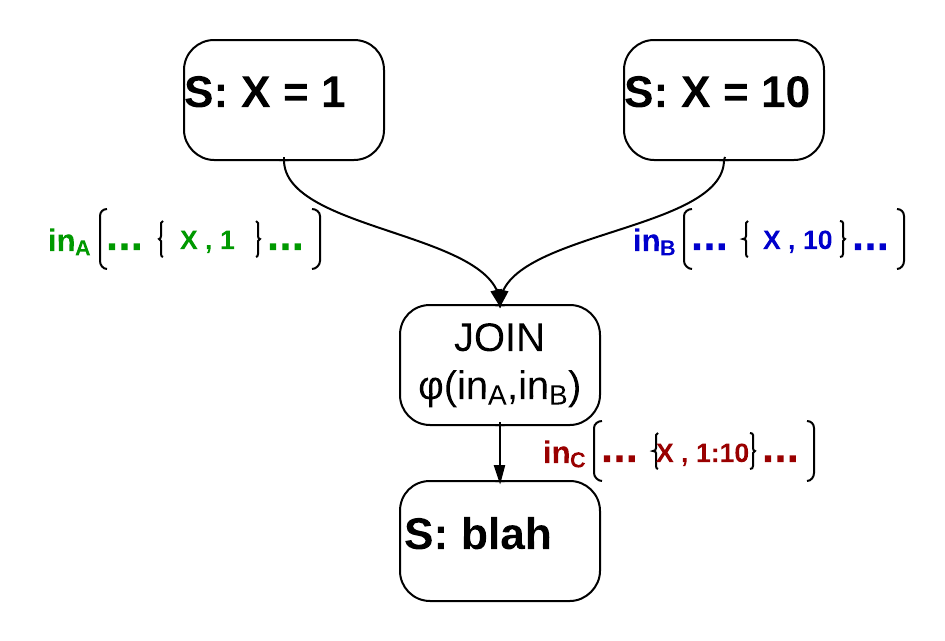
\includegraphics[width=0.4\textwidth]{MergeNode}
\caption{A Range analysis merge. Unlike constant propagation, $x$ becomes all possible values at $in_c$ and not top. }
\label{RngMergeNode}
\end{figure}
There are two complications with this analysis which are described as follows;\\
\begin{itemize}
\item{\textbf{Flow functions:} Flow functions must assume range tuples and calculate the maximum tuple for each statement.}
\item{\textbf{Loop detection:} Given that the range of numbers is infinite, for termination a heuristic loop detector should be added to the join. We will elaborate later in the document.}
\end{itemize}
\subsection{Lattice \& Flow Functions}
for range analysis, we decompose all variable types to two numerical primitives of \emph{int} and \emph{float} that correspond to LLVM's constant and register types \emph{IntxTy} and \emph{FloatTy}. This bounds range to the \emph{max} and \emph{min} of these types, but it is still large enough that we need the heuristic loop detector mentioned earlier. Any constant or operand that cannot be cast to a \emph{int} or \emph{float} cannot have a range and so will be outside of the lattice domain.\\
We introduce the concept of:
$$ X \ra \{min,max\} \in Z^2$$
to represent the range of a variable $X$ given the set of variables $Z$, where $min$ is the lowest value X could be and $max$ is the highest. \\
Furthermore we define all constants $N$ to be a range of 1 using similar notation: 
$$ N \ra\{n,n\} \in \mathbb{R}$$
This means that constants may be assigned to variables, as is necessary for analysis and in actual code. \\
\subsubsection{Lattice and the Join}
The set join is complicated for range analysis so extra discussion is provided after defining the lattice.
Let $Vars$ be the set of C++ variables present in the program. Given two flows $F,F'$, we have :
\begin{align*}
F \sqsubseteq & F'  & \lra & & F \subseteq F' \\
\top & & \lra & & \{ X \ra \{-\infty; +\infty\} | \forall X \in Vars \}\\ 
\bot & & \lra & & \emptyset \\ 
F \sqcup F' & & \lra & & (F \ra h(F)) \cup (F'\ra h(F')) \\
F \sqcap F' & & \lra & & F \cap F'
\end{align*}

\textbf{The Join}\\
$h(X)$ is a loop detection heuristic. 
\begin{figure}[here]
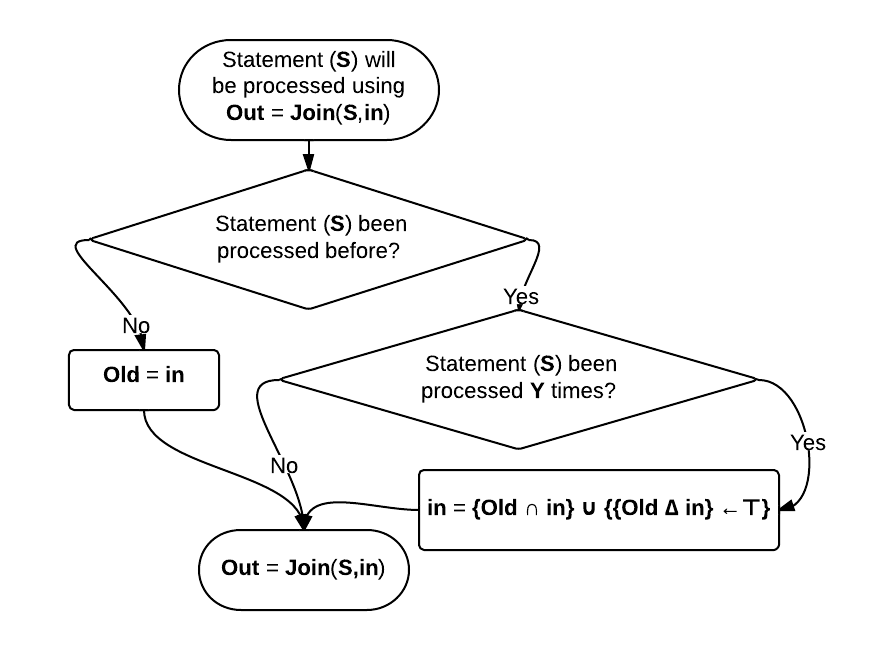
\includegraphics[width=0.4\textwidth]{loopDetector}
\caption{The range analysis Join. A heuristic is used to quickly reach a fixed point for the loop body statements.}
\label{LoopDetectHeuristic}
\end{figure}

The heuristic is described a flow chart in Figure~\ref{LoopDetectHeuristic}
The heuristic can guarantee correctness but depending on Y it may can give very imprecise information. A higher $Y$ increasing the likelihood the loop control will reach its upper bound, which increases precision since a local fixed point occurs and statements from the loop body will not be added to the work list at this point. We were not aggressive with $Y$ because of an exponential analysis run-time cost. We reason a cost factor of $\bar{Loops} \times \bar{BodyLength}$ meaning $Y$ should not be too high for scalable analysis and choose 3 to demonstrate our heuristic concept. We considered a more sophistic range detection based on taken/untaken predecessor blocks, but unable to successfully implement this. More detail is provided in the implementation section.

\subsubsection{Flow Functions}
We list the instructions covered by our our range analysis in Table~\ref{rangeAnalysisTable}. For each instruction, we define $F_{IN}$ and $F_{OUT}$ as the input and output of the flow functions for each instruction, respectively. Table~\ref{rangeAnalysisTable} is a selection of flow functions to show the supported binary arithmetic and logical statements of our range analysis. We do not list a flow function for every operand type permutation (possible operand combinations of constants, $N$ and variables $X$). We do not need to do so since constants and variables exist in our domain ($\bot \subseteq n \subseteq \top \forall N$ and $\bot \subseteq x \subseteq \top \forall X$) so either $A$ or $B$ or both in Table~\ref{rangeAnalysisTable} may be substituted with $N$. For the same reason we also do not list different flow functions for The primitive types \emph{FloatTy} and \emph{IntxTy}. The flow functions all use a binary operator substitution, \emph{Combo(A,B,Op)} defined under Table~\ref{rangeAnalysisTable} to exhaustively find the maximum range of any binary operator. This could be optimized for adding and shifting cases, but we feel this would obfuscate the flow functions.\\
Besides the binary operators we define flow functions for pointer de-reference. Because our pass has no access to points-to information, to be safe our pass simply returns max range to either the assigned variable or the set of variables.  %All upper case literals are variables and all lower case literals are constants. We use shorthand for readability of our flow functions, which is expanded below the main table. 
%{\footnotesize
%\begin{align*} 
%& X \la A + B  & : & & F_{OUT} = F_{IN} - \{X \ra *\}\cup \{ X \ra \{min(Combo(A,B,+)); max(Combo(A,B,+)) \} | A \in Vars \wedge B \in Vars \} \\
%& X \la A - B & : & & F_{OUT} = F_{IN} - \{X \ra *\}\cup \{ X \ra \{min(Combo(A,B,-)); max(Combo(A,B,-)) \} | A \in Vars \wedge B \in Vars \} \\
%& X \la A \times B & : & & F_{OUT} = F_{IN} - \{X \ra *\}\cup \{ X \ra \{min(Combo(A,B,\times)); max(Combo(A,B,\times)) \} | A \in Vars \wedge B \in Vars \} \\
%& X \la A \div B & : & & F_{OUT} = F_{IN} - \{X \ra *\}\cup \{ X \ra \{min(Combo(A,B,\div)); max(Combo(A,B,\div)) \} | A \in Vars \wedge B \in Vars \} \\
%& X \la A MOD B & : & & F_{OUT} = F_{IN} - \{X \ra *\}\cup \{ X \ra \{min(Combo(A,B, \%)); max(Combo(A,B,\%)) \} | A \in Vars \wedge B \in Vars \} \\
%& X \la A LSHL B & : & & F_{OUT} = F_{IN} \cup \{W \ra Z | X \ra W \wedge Y \ra Z \} \\
%& X \la A LSHR B & : & & F_{OUT} = F_{IN} \cup \{X \ra Z | Y \ra W \wedge W \ra Z \} \\ 
%& X \la A ASHR B & : & & F_{OUT} = F_{IN} \cup \{X \ra Z | Y \ra W \wedge W \ra Z \} 
%\end{align*}

%where:
%}%

\begin{table*}[t]
\centering
\caption{Range analysis flow functions}
\begin{tabular}{| c | l | }
\hline
\multicolumn{1}{c}{\textbf{Statement}} & 
  \multicolumn{1}{c}{\textbf{Flow function}}\\\hline
$X \la A + B$  & \shortstack{$F_{OUT} = F_{IN} - \{X \ra *\}\cup$ \\$\{ X \ra \{min(Combo(A,B,+)); max(Combo(A,B,+)) \} | A \in Vars \wedge B \in Vars \}$} \\
$X \la A - B$  & \shortstack{$F_{OUT} = F_{IN} - \{X \ra *\}\cup$ \\$\{ X \ra \{min(Combo(A,B,-)); max(Combo(A,B,-)) \} | A \in Vars \wedge B \in Vars \}$} \\
$X \la A \times B$  & \shortstack{$F_{OUT} = F_{IN} - \{X \ra *\}\cup$ \\$\{ X \ra \{min(Combo(A,B,\times)); max(Combo(A,B,\times)) \} | A \in Vars \wedge B \in Vars \}$} \\
$X \la A \div B$  & \shortstack{$F_{OUT} = F_{IN} - \{X \ra *\}\cup$ \\$\{ X \ra \{min(Combo(A,B,\div)); max(Combo(A,B,\div)) \} | A \in Vars \wedge B \in Vars \}$} \\
$X \la A \% B$  & \shortstack{$F_{OUT} = F_{IN} - \{X \ra *\}\cup$ \\$\{ X \ra \{min(Combo(A,B,\%)); max(Combo(A,B,\%)) \} | A \in Vars \wedge B \in Vars \}$} \\
$X \la A LSHL B$  & \shortstack{$F_{OUT} = F_{IN} - \{X \ra *\}\cup$ \\$\{ X \ra \{min(Combo(A,B,LSHL)); max(Combo(A,B,LSHL)) \} | A \in Vars \wedge B \in Vars \}$} \\
$X \la A LSHR B$  & \shortstack{$F_{OUT} = F_{IN} - \{X \ra *\}\cup$ \\$\{ X \ra \{min(Combo(A,B,LSHR)); max(Combo(A,B,LSHR)) \} | A \in Vars \wedge B \in Vars \}$} \\
$X \la A ASHR B$  & \shortstack{$F_{OUT} = F_{IN} - \{X \ra *\}\cup$ \\$\{ X \ra \{min(Combo(A,B,ASHR)); max(Combo(A,B,ASHR)) \} | A \in Vars \wedge B \in Vars \}$} \\
$X \la *Y$ & $F_{OUT} = F_{IN} - \{X \ra *\}\cup \{X \ra \{-\infty,+\infty\}\}$\\
$*X \la Y$ & $F_{OUT} = F_{IN} - \{Z \ra * \forall Z\in Vars\}\cup \{Z \ra \{-\infty,+\infty\} \forall Z\in Vars\}\}$\\
\hline

\end{tabular}
\label{rangeAnalysisTable}

where: ${M[m_1:m_4]} \gets Combo(A,B,Op) \lra ((A_{[0]} Op B_{[0]}),(A_{[0]} Op B_{[1]}),(A_{[1]} Op B_{[0]}),(A_{[1]} Op B_{[1]}))$ 
\end{table*}

%Notice that scope of instructions covered could be larger and these out-of-scope instructions fall into two categories. Instructions such as $X \la c$ (where $X$ is a pointer variable) are explicitly forbidden in C++ language. Instructions such as $*X \ra *Y$ are legitimate candidates but where not implemented because of time constraints. 
\subsection{Implementation}
The range analysis pass is performed after a "\textbf{mem2reg}" pass. Without mem2reg, the pass must resolve variables from load and store instructions along with other complications.\\
Using mem2reg has a disadvantage that source code variables do not correspond to the .ll code input to our range analysis. We were unable to robustly transpose source code variables to our range analysis input, so our range analysis could not implement bounds checking.\\
Because of this limitation we were not aggressive with our join heuristics and chose a simple three statement counter to demonstrate the concept of heuristic loop detection for balancing pass execution time and information preciseness.\\
We provide an example snipped  for a flow function but focus discussion on our join operator. This is because our flow functions follow a similar template and because the join heuristic is responsible for a practical range analysis' achievable precision.\\
The multiplication flow function is as follows:
%Each mathematical instruction is identified by its corresponding C++ and LLVM code snippets, which are available on table \ref{pointerAnalysisTable}. When the \code{Flow* executeFlowFunction()} is executed, the instruction's opcode is parsed and the computation performed is selected using switch statements as follows :

\begin{lstlisting}[caption=Range analysis flow functions, label=PAFF]
DomEl getOpRng(DomEl a, 
               DomEl b, 
               unsigned opcode)
{
...//Declarations, sanity checks etc.
  switch(opcode) 
  {
  	...
    case MUL:

      Comb[0] = a.lower * b.lower;
      Comb[1] = a.lower * b.upper;
      Comb[2] = a.upper * b.lower;
      Comb[3] = a.upper * b.upper;
      resRange.lower = Comb[0];
      resRange.upper = Comb[0];
      while(i < 4)
      {
        if(Comb[i] < resRange.lower)
    	         resRange.lower = Comb[i];
        if(Comb[i] > resRange.upper)
    	         resRange.upper = Comb[i];
        i++;
      }
      break;
    ...
  }//end case
  return resRange;
}
\end{lstlisting}

The Join operation is composed of three parts:
\begin{itemize}
\item{\textbf{Heuristic loop detection $h(in)$: }Keep copies of the first mappings for each statements. Output is consumed by the join operation.}
\item{\textbf{Join sets $\cup$: }The set wise join operation}
\item{\textbf{Join elements: }A range analysis specific element wise join taking the maximum possible range of two domain elements}
\end{itemize}

Besides the set join, $\cup$, we provide code snippets below. Set join is omitted since it is similar to other analysis.\\


 \begin{lstlisting}[caption=Heuristic loop detector $h(in)$, label=PAFF]
Flow* FF(Flow *in, Ins *inst, int S_id) 
{
 if(nodeCount.find(S_id)!=nodeCount.end())
 {
    //Y is set to 3
    if(nodeCount[S_id].VisitCtr >= 3)
    {
      ...
      //Set ranges that changed to TOP
      DifToTop(in, 
               nodeCount[S_id].nodeSet);
      //*in is modified
      return(in);
    }
    nodeCount[S_id].VisitCtr = 
              (nodeCount[S_id].VisitCtr+1);
  }
  else
  {
    ...
    nodeState thisNodeState;
	thisNodeState.VisitCtr = 1;
	thisNodeState.nodeSet = in;//'Old'
	nodeCount[NodeId] = thisNodeState;
  }

 \end{lstlisting}
 
 \begin{lstlisting}[caption=Per domain element join, label=PAFF]
DomEl JoinEls(DomEl* A, DomEl* B)
{
  DomEl maxAB;

  maxAB.lower = (A->lower <= B->lower) ? 
                       A->lower : B->lower;
  maxAB.upper = (A->upper >= B->upper) ? 
                       A->upper : B->upper;
  return maxAB;
}
 \end{lstlisting}

\section{Conclusion}

The project was completed succesfully . Learning outcomes were a working understanding of LLVM optimiser passes. We are capable of transforming and instrumenting code. We have developed an efficient method to develop, test and debug the LLVM source tree with a debug api and symbol indexed code base via the eclipse CDT. Understanding how to instrument code has provided a powerful tool for analysis of any optimisation heuristics applied by other opt passes. Instrumentation will allow us to both formulate and test heuristics based on the performance of compiled code.\\
To conclude, this project has provided us with a solid foundation for the second upcoming project for CSE 231


\end{document}
